\documentclass[titlepage]{article}
\usepackage{graphicx}
\usepackage[tbtags]{amsmath}

\begin{document}

\title{Experiment 2: Mini Report}
\author{Tian Ye \\ \\ UID: 704931660 \\ \\ TA: Wen Li Wen \\ \\ Lab Partners: \\ \\ Matthew Barba, Dong Han,\\ \\ Chris Ong, Edward Xie \\ \\ Lab 8 Tuesday 6:00 PM}
\date{October 17th, 2017}

\maketitle

\begin{figure}[!htbp]
    \centering
    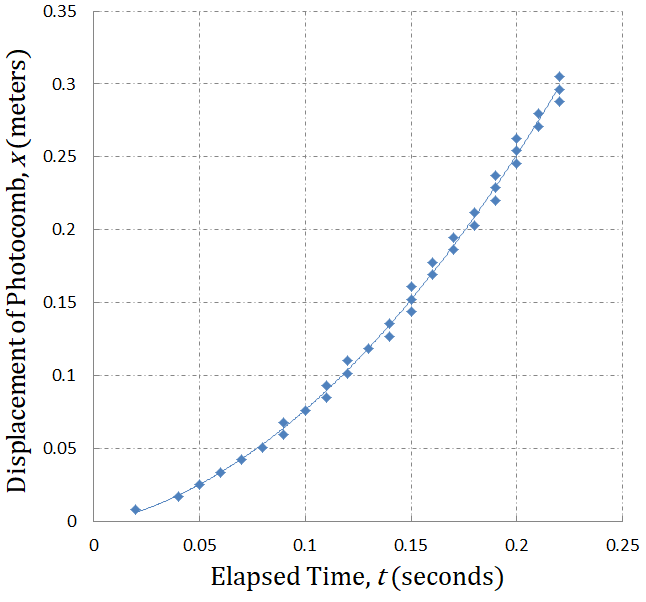
\includegraphics[width=4.0in]{Figure.png}
    \caption{Effect of gravitational constant, $g$, on photocomb displacement. The independent variable is elapsed time, measured in seconds, and the dependent variable is displacement of the photocomb, measured in meters. Each blue diamond represents the displacement of the photocomb and the point in time at which said displacement occurred. The solid blue line is a quadratic regression fit line to the data, $\Delta x = x_0 + v_0t + \frac{1}{2}at^2$, with fit parameters of $x_0 = (-0.0018 \pm 0.0049)$ m, $v_0 = (0.2988 \pm 0.0800)$ m/s, and $a = (9.6904 \pm 0.2987)$ m/s$^2$. The regression curve indicates that $g$ is a constant with a value of $9.6904 \pm 0.2987$ m/s$^2$.}
\end{figure}

Taking the output of the photogate sensor, we are provided with the elapsed time at which every single "block", or slit in the comb, allowed the LED in the photogate to reach the sensor at the other side and consequently register an input. To obtain displacement at each given elapsed time data point, we multiply $\lambda$, the distance between the leading edge of one slit to the leading edge of the next slit, and multiply it by $n$, the number of the associated elapsed time data point. For example, $n$ for the first data point would be 1, the second 2, etc.

Taking acceleration due to gravity being constant, a quadratic regression can then be performed on the data to solve for $g$. Figure 1 represents the plot of displacement vs elapsed time for the photocomb with the quadratic regression line, given in the form:

\begin{align}
     \Delta x = x_0+v_0t+\frac{1}{2}at^2
\end{align}

The regression tool outputs an equation with the form of $y = ax^2 + bx + c$, which when compared with Equation 1 above, allows us to see that $y = \Delta x, x = t, a = \frac{1}{2}a, b = v_0,$ and $c = x_0.$ Therefore, we can calculate the magnitude of acceleration on the photogate comb, in this case being $a = g = 9.6904$ m/s$^2$.

This analysis of $g$, however, is incomplete as it does not account for uncertainties, both systematic and statistical. Using again Excel's regression tool, we solve for the statistical uncertainty in the quadratic coefficient, being $\pm$ 0.2987 m/s$^2$. 

To solve for systematic uncertainty on the other hand requires taking into account the uncertainty of $\lambda$, being $\pm$ 0.5 mm. Using $\delta\lambda$ to maximize and minimize $g$, we can then solve for the systematic uncertainty component of $g$ using the following equation:

\begin{align}
     \delta g = \frac{g\textsubscript{max} - g\textsubscript{min}}{2}
\end{align}

From this, we find the systematic uncertainty of $g$ to be $\pm$ 0.0058 m/s$^2$. When we compare the values of the systematic uncertainty of $g$ to the statistical uncertainty of $g$, we find that the systematic uncertainty is approximately 50 times smaller than the statistical uncertainty. This allows us to ignore the effect of the systematic uncertainty, as the value of the systematic uncertainty would be truncated when taking into account significant figures.

This allows us to conclude that the acceleration due to gravity for this particular trial of the photocomb drop is $g = 9.69$ $\pm$ 0.30 m/s$^2$.

\section*{}
Length of Caption: 108 words
\subsubsection*{}
Length of Text: 377 words

\end{document}
T